\section{Approach}
\label{chap:approach}

As seen in \hyperref[chap:related_work]{section \ref{chap:related_work}}, research proposes various theoretical frameworks and implementations in the area of argumentation mapping. This section introduces the concept of ``DialogMap'' and gives information about the context and background of the developed prototype (sub-section \ref{sub:dialogmap}), describes general concepts of the implemented prototype (\hyperref[sub:design]{sub-section \ref{sub:design}}) and lay out implementation details (\hyperref[sub:implementation]{sub-section \ref{sub:implementation}}).

\subsection{DialogMap}
\label{sub:dialogmap}

Following the concept of Rinner's Argumentation Map \cite{Rinner_ArgumentationMaps} and the idea of supporting public deliberation through spatially enhanced dialogs, the concept of DialogMap was developed. Following the recommendations and suggestions of the research presented in \hyperref[subchap:gis_stuff]{section \ref{subchap:gis_stuff}}, a set of functional and non-functional requirements have been derived.\\
DialogMap is a spatial online discussion platform to support geodeliberative dialogs perfomed by citizen initatives \cite{Cai2009_spatial_annotation_deliberation}. It enables its users to make explicit spatial references in their discussion contributions to clarify denotation of spatial relationships. This is achieved by allowing the interlinking of one or multiple words with a location or area on the map of the application \cite{Rinner_ArgumentationMaps}. It is possible to create multiple connections between locations in one contribution, as well as referring to locations created in the context of another contribution \cite{Kessler2005_ArgumentationMapPrototype,Voss2004_Evolution_PGIS,you2009_participatory_map_based,Cai2009_spatial_annotation_deliberation} to allow more fine grained references. This creates the possibility for many-to-many connections between locations and words. It is also possible to create multiple hyperlinks on words or multiple words in the contributions' text. The creation of the references and the text can occur in any order \cite{Voss2004_Evolution_PGIS}. It was found that through allowing spatial references, exchange of information can be made more efficient \cite{Cherubini2007_shared_maps}.\\
Contributions comprise not only of a text with spatial references and hyperlinks, but is composed of multiple other attributes and properties \cite{Longueville2010_community_based_geoportals_web20,Kessler2005_ArgumentationMapPrototype,Kessler2005_Conflict_Resolution}. Users are able to specify tags and a category and to attach an image to each contribution \cite{Tang2005_PPGIS_discussion_forum,zhao2006geodf,you2009_participatory_map_based,Cai2009_spatial_annotation_deliberation} to support their statements in their contributions. The tags and category of the contribution affect the visual appearance of the geo-features created in its context.\\
DialogMap favors linear dialogs by structuring the contributions chronologically \cite{Cherubini2007_shared_maps,you2009_participatory_map_based}. Contributions can be made without context or as a reply to a contribution. It is possible to edit contributions along with its properties and created references. It is also possible to mark contributions as deleted, which results in a visual marking of the textual representation as well as the fading of the geo-features created in the context of the contribution \cite{Hopfer2007_Communication}. This further supports the linearity of the structured discussions.\\
Creation of contributions is only allowed after authenticating to the system. Users can either register an user account with a e-mail password combination or authenticate themselves through a third party authentication provider \cite{Sani2011_Scalable_Argumap,chun2014usability}.\\
The user interface of DialogMap features a map and an area to display the textual representations of a contribution. Spatial and textual representations of the contributions are interlinked by a two way highlighting to indicate the relationships between geo-features and contributions \cite{Cai2009_spatial_annotation_deliberation,Sidlar2009-AssessmentMapGeocollaborationTool}.\\
DialogMap allows to filter and search for contributions by categories, tags and by free text. This enables users to create their own contribution overviews \cite{Voss2004_Evolution_PGIS,you2009_participatory_map_based}, and allows users to see gaps and thoroughly covered areas \cite{Hopfer2007_Communication}.\\
The importance of an easy user interface was mentioned by many authors \cite{Rinner2009_Web2_argumap,Jankowski2005_community_based_pgis,Tang2005_PPGIS_discussion_forum,zhao2006geodf,you2009_participatory_map_based}. As users are likely non-technical \cite{Cai2009_spatial_annotation_deliberation}, the user interface should not discriminate them, thus suppressing participation \cite{Carver2001_PPGIS_Cyberdemocracy}.\\
An important technical aspect of the conception and development of an spatial discussion platform is to plan it flexible enough to be reused for multiple use cases \cite{Kessler2005_Conflict_Resolution,Kessler2005_ArgumentationMapPrototype,Sani2011_Scalable_Argumap}. This was adequately honored through the Model-view-controller pattern in both the backend and frontend. Another recommendation was, to make the architecture modular, to make the application scalable \cite{Sani2011_Scalable_Argumap} to serve many users at the same time.

In order to test the initial idea of supporting public deliberation through spatially enhanced dialogues, a working prototype was developed. Starting from the concept of DialogMap, a first prototypical application was developed. The development was done in an iterative and agile approach. The creation of working iterations of the DialogMap concept made early feedback possible. The possibility to evaluate the concept in a real world use case with users of scientific citizen initiatives presented itself early in the development process. The further development was then conducted with with practical advice from members of one scientific citizens' initiative. Their input ranged from general suggestions to opinions of specific features. Thus, the following sections describe the distinct outcome of their input to the developed prototype.

%``Integrated user interface'', ``Structured discussion'', ``Common (Web)mapping functions'', ``Integrated database, many-to-many relationships'', ``Access control, security'' and ``Customization by Provider''. \cite{Kessler2005_ArgumentationMapPrototype}

%Recommendations for implementing PPGIS \cite{Carver2001_PPGIS_Cyberdemocracy} \cite{Voss2004_Evolution_PGIS}

\subsection{Application Design} % and features
\label{sub:design}

Internally, the prototype uses few data models. In the configuration used for this thesis, a contribution contains a title, description, two categories, a tags field, a favored counter, an optional time restriction field for start and ending times, an optional image, an optional reference to a parent contribution and optional references to child contributions. The parent and child contribution references create a simple parent-child connection between contributions, as children inherit the categories, tags, time restriction and title. A contribution serves both as a topic and as response to a topic. A contribution also contains references to features, references to feature references and references to URLs.\\
Features are geospatial entities with a location, a reference to its contribution and properties for styling\footnote{\url{https://github.com/mapbox/simplestyle-spec}}.\\
Feature references contain a title, which can differ from the original title of the feature and a reference to a feature. URL references contain hyperlinks and a description of the hyperlink. The description of a contribution contains the text typed by a user with specially encoded references to features, URL references and feature references. Additionally, each contribution stores the ids of the users who favored it.\\
Users can create contributions in the manner of creating topics or writing responses to existing topics. Users have an e-mail address and a name. \hyperref[fig:data_structure]{Figure \ref{fig:data_structure}} depicts a generalized data structure diagram.

\begin{figure}[!h]
    \centering
    \includegraphics[width=1\columnwidth]{images/data_structure}
    \caption{Schema of the underlying data structure of the prototype. Time and id fields are omitted for brevity.}
    \label{fig:data_structure}
\end{figure}

The front page of the prototype consists of a map with a sidebar. This allows the user to see both the spatial and textual representations of a contribution at one glance. The right hand sidebar contains the input form for new contributions, filter options, sorting order selector and the list of contributions. The input form consists of input fields for title, categories, time restriction, image and description. The description field allows the creation of spatial features and URL/feature references through connecting words with spatial representations or URLs. (See \hyperref[fig:screenshot_create]{Figure \ref{fig:screenshot_create}})\\
A text area for arbitrary text and multiple checkboxes allow to restrict the listed contribution as well as the geo-features displayed in the map. It is also possible to change the sorting order of the list of contribution through a drop down field. \hyperref[fig:screenshot_filter]{Figure \ref{fig:screenshot_filter}} depicts the expanded filter with several checkboxes enabled.

\begin{figure}[!h]
    \centering
    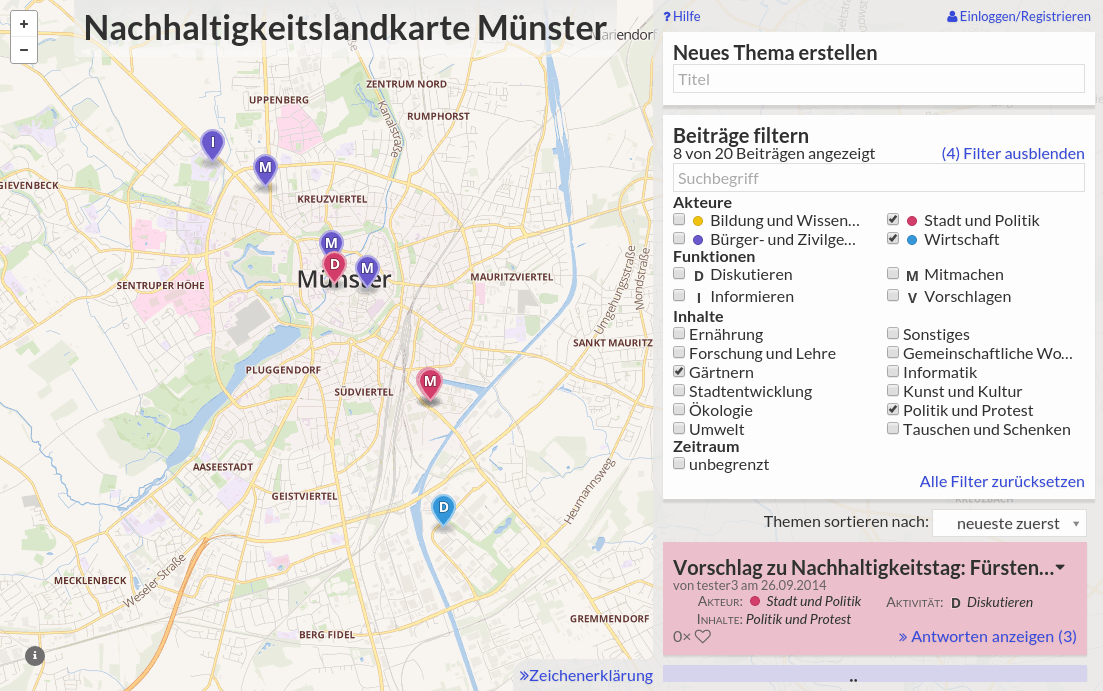
\includegraphics[width=1\columnwidth]{images/screenshot_filters}
    \caption{\textit{DialogMap} with expanded filter.}
    \label{fig:screenshot_filter}
\end{figure}

The list of contributions contains colored rectangles representing the different topics. Each rectangle contains the title, time of writing, name of the author, categories, tags and the amount of times the contribution has been favored by users. It also contains a link which navigates to the replies written to the topic. A click on the contribution rectangle expands it vertically, revealing the description of the current topic.\\
After clicking the ``reply'' link, only the selected topic and replies are shown in the sidebar in a chronological order. In this view, each contribution shows the description by default as well as author and time and date of writing. The author of the contribution is able to edit and delete the contribution. Upon deletion, the user can enter a reason for deletion, which then will be displayed below the deleted contribution. The deletion is not destructive. The contribution as well as features created for the contribution are marked visually as deleted. Other users are able to favor contribution to show interest or agreement.

\begin{figure}[!h]
    \centering
    \includegraphics[width=1\columnwidth]{images/screenshot_create}
    \caption{Input form of \textit{DialogMap} for creating a new topic.}
    \label{fig:screenshot_create}
\end{figure}

The map view contains a base map and several markers and polygons in different colors and different icons in case of markers. These relate to the contributions and are connected through the references in the description of the contributions. Which spatial features are displayed is determined through the state of the sidebar. In the topics overview, only the features created for the starting contributions are displayed in order to prevent cluttering of the view-port. When only a topic and its replies are displayed in the sidebar, all features related to the topic and its replies are shown on the map.\\
To emphasize the relationship between a contribution and its spatial features, a two way highlighting has been implemented. Hovering over either a contribution-box, marked word or spatial feature on the map triggers visual highlighting on all related contributions, marked words and spatial features. This allows to quickly grasp the relationship between features and contributions. \hyperref[fig:screenshot]{Figure \ref{fig:screenshot}} shows an active highlighting initiated through a mouseover over a marker.\\
Users are able to use either traditional sing-up/sign-in methods or sign-in through different social log-in providers to authenticate to the system.

\begin{figure}[!h]
    \centering
    \includegraphics[width=1\columnwidth]{images/screenshot}
    \caption{Screenshot of the front page of \textit{DialogMap} with active highlight of a contribution and spatial feature.}
    \label{fig:screenshot}
\end{figure}

\subsection{Implementation}
\label{sub:implementation}
\textit{DialogMap} has been implemented as a single-page web application using AngularJS\footnote{\url{http://angularjs.org/}} and Ruby on Rails\footnote{\url{http://rubyonrails.org/}}. The single-page structure was chosen in order to provide the user with a clear navigation between the overview and contribution answers. This also allows for a seamless browsing experience without full reloads of the page. AngularJS is a JavaScript framework with features like templating, two-way binding and DOM manipulation. It follows the model-view-controller pattern in order to bring server side paradigms to client-side development. AngularJS was chosen because of its popularity, extensibility and high number of available libraries. It also enables to wrap existing JavaScript libraries to be used in AngularJS context.\\
The mapping library Leaflet\footnote{\url{http://leafletjs.com/}} serves as base for displaying base maps and geospatial data. The user-facing web page was developed using tools like CoffeeScript\footnote{\url{http://coffeescript.org/}}, Haml\footnote{\url{http://haml.info/}} and Sass\footnote{\url{http://sass-lang.com/}} to speed up the development. The web page was developed with all major browsers in mind.\\
On the server side, components were developed using the Ruby on Rails framework with PostgreSQL\footnote{\url{http://www.postgresql.org/}}/PostGIS\footnote{\url{http://postgis.net/}} as data storage. Ruby on Rails, originally a full-stack model-view-controller web framework, is used as a JSON serving application logic. It was chosen because of its maturity and high number of available libraries. Front- and backend of the prototype communicate in REST-API\footnote{Representational State Transfer Application programming interface} like manner. This allows for easily replaceable front- and backend application stacks.\\
Figure \ref{fig:screenshot} shows the front page of the prototype with an active two way highlight.\\
Without the extensive use of open source software and code, development would have taken much longer. The source code as well as installation instructions are accessible online through GitHub\footnote{\url{https://github.com/ubergesundheit/dialogmap}}.




